\documentclass[11pt,a4paper]{article}

\usepackage{../../templates/style}

\begin{document}

\begin{problem}{PERIODNI}{standard input}{standard output}{5 second}{32 megabytes}

Luka รู้สึกเบื่อในคาบเรียนวิชาเคมี ดังนั้น เขาจึงจ้องมองไปยังตารางธาตุเคมีขนาดใหญ่ที่แขวนอยู่ที่กำแพงตรงเหนือกระดานดำและเพื่อเป็นการฆ่าเวลา   Luka จึงตัดสินใจที่จะสร้างตารางธาตุที่สมบูรณ์ของเขาขึ้นมาเอง ซึ่งแตกต่างจากอันที่แขวนอยู่ในห้องเรียน

ตาารางของเขาประกอบด้วย $N$ คอลัมน์และในแต่ละคอลัมน์จะมีค่าความสูงของมันเอง โดยทุกคอลัมน์จะเรียงต่อกันที่ด้านล่างของตาราง ดังเช่นที่แสดงในรูปตัวอย่างด้านล่างนี้   หลังจากที่เขาวาดตารางของเขาขึ้นมาแล้ว เขาต้องการที่จะเติมธาตุต่าง ๆ ลงในช่องว่างของตาราง เริ่มแรกเขาตัดสินใจที่จะเติมแก๊สเฉื่อยจำนวน $K$ ธาตุลงไป   และเขาต้องการที่จะใส่มันลงไปในตารางโดยที่จะต้องไม่ให้มีแก๊สเฉื่อย $2$ แก๊สใด ๆ อยู่ใกล้กันและกันในตาราง

รูปสี่เหลี่ยม $2$ รูปใด ๆ ในตารางจะถือว่าอยู่ใกล้กันและกัน   ถ้ารูปสี่เหลี่ยม $2$ รูปนั้นอยู่ในคอลัมน์หรือแถวเดียวกันและต้องมีรูปสี่เหลี่ยมอื่น ๆ คั่นระหว่างรูปสี่เหลี่ยมทั้งสองนั้นด้วย  ในตัวอย่างด้านล่างนี้ รูปสี่เหลี่ยม “a” ถือว่าไม่อยู่ใกล้ซึ่งกันและกัน   ในขณะที่รูปสี่เหลี่ยม “b” ถือว่า อยู่ใกล้ซึ่งกันและกัน

\begin{figure}[!h]
\centering
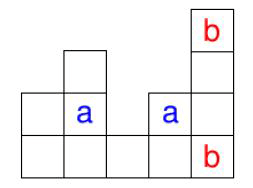
\includegraphics[width=0.7\textwidth]{../latex/img/1098/1098.png}
\end{figure}

\bigskip
\underline{\textbf{โจทย์}}  จงเขียนโปรแกรมเพื่อรับค่า $N, K$ และ ค่าความสูงในแต่ละ $N$ คอลัมน์   แล้วคำนวณหาจำนวนวิธีทั้งหมดที่ Luka สามารถเติมแก๊สเฉื่อยลงไปในตารางได้   ซึ่งค่าผลลัพธ์ที่ได้นี้อาจมีค่ามาก   ดังนั้นให้แสดงผลข้อมูลส่งออกโดยมอดุโลค่านี้ด้วย $1\,000\,000\,007$


\InputFile

\textbf{บรรทัดแรก}   ประกอบด้วยเลขจำนวนเต็ม $N$ และ $K$ ซึ่งคั่นกันด้วยช่องว่าง   โดย  $N$ และ $K$ มีค่าดังนี้ $1 \leq N \leq 500; 1 \leq K \leq 500$ ซึ่งหมายถึงจำนวนของคอลัมน์ในตารางของ Luka และจำนวนของแก๊สเฉื่อย ตามลำดับ

\textbf{บรรทัดที่สอง}   ประกอบด้วยเลขจำนวนเต็มบวก $N$ ค่าและแยกกันโดยใช้ช่องว่าง   ซึ่งหมายถึงค่าความสูงในแต่ละคอลัมน์จากซ้ายไปขวา   โดยค่าความสูงเหล่านี้จะมีค่ามากที่สุดคือ $1\,000\,000$



\OutputFile

\textbf{มีบรรทัดเดียว} ให้แสดงผลข้อมูลส่งออกด้วยผลลัพธ์ของจำนวนวิธีทั้งหมดที่ Luka สามารถเติมแก๊สเฉื่อยลงในตารางได้มอดุโลด้วย $1\,000\,000\,007$

\Examples

\begin{example}
\exmp{3 3
2 1 3}{2}%
\exmp{4 1
1 2 3 4}{10}%
\exmp{5 2
2 3 1 2 4}{43}%
\end{example}

\Scoring

\textbf{จะได้รับคะแนน $40$ เปอร์เซ็นต์ของคะแนนทั้งหมด}   ถ้าตัวเลขทั้งหมดในข้อมูลนำเข้ามีค่าน้อยกว่า $15$

\textbf{จะได้รับคะแนน 70 เปอร์เซ็นต์ของคะแนนทั้งหมด}   ถ้าตัวเลขทั้งหมดในข้อมูลนำเข้ามีค่าน้อยกว่า $100$
  
\Source

COCI 2008/2009, Contest \#4 – January 17, 2009

\end{problem}

\end{document}